\documentclass{standalone}
\usepackage{tikz}
\usepackage{ctex,siunitx}
\setCJKmainfont{Noto Serif CJK SC}
\usepackage{tkz-euclide}
\usepackage{amsmath}
\usetikzlibrary{patterns, calc}
\usetikzlibrary {decorations.pathmorphing, decorations.pathreplacing, decorations.shapes,}
\begin{document}
\small
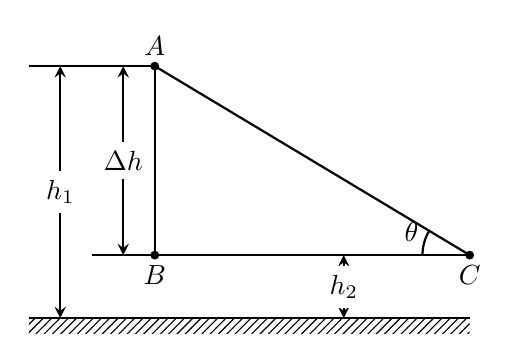
\begin{tikzpicture}[>=stealth,thick,scale=0.8]
  \fill [pattern = north east lines] (-1,-.25) rectangle (6,0);
  \draw (-1,0)--(6,0);
  \draw (1,4)node[above]{$A$}--(1,1)node[below]{$B$}--(6,1)node[below]{$C$};
  \fill (1,4) circle(2pt);\fill (1,1) circle(2pt);\fill (6,1) circle(2pt);
  \draw[<->](4,0)--node [fill=white]{$h_2$}(4,1);
  \draw[<->](.5,1)--node [fill=white]{$\Delta h$}(.5,4);
  \draw[<->](-.5,0)--node [fill=white]{$h_1$}(-.5,4);
  \draw (-1,4)--(1,4);
  \draw (0,1)--(1,1);
  \draw (1,4)--(6,1);
  \draw (6-.75,1) arc (180:150:.75)node[left]{$\theta$};
\end{tikzpicture}
\end{document}